\documentclass[a4paper,10pt]{article} % Default font size and paper size

\usepackage{multirow}
\usepackage{hyperref}
\usepackage{url,parskip} % Formatting packages
\usepackage{graphicx}

\usepackage[usenames,dvipsnames]{xcolor} % Required for specifying custom colors

% Espaiat entre línies
%\onehalfspacing
\usepackage{array}
\usepackage{ragged2e}
\newcolumntype{L}[1]{>{\raggedright\let\newline\\\arraybackslash\hspace{0pt}}m{#1}}
\newcolumntype{C}[1]{>{\centering\let\newline\\\arraybackslash\hspace{0pt}}m{#1}}
\newcolumntype{R}[1]{>{\raggedleft\let\newline\\\arraybackslash\hspace{0pt}}m{#1}}

% To reduce the height of the top margin uncomment: \addtolength{\voffset}{-1.3cm}
\usepackage[left=2.5cm,right=2.5cm,top=2cm,bottom=2.5cm]{geometry}
\usepackage{hyperref} % Required for adding links	and customizing them
\definecolor{linkcolour}{rgb}{0,0.2,0.6} % Link color
\hypersetup{colorlinks,breaklinks,urlcolor=linkcolour,linkcolor=linkcolour} % Set link colors throughout the document

\usepackage{titlesec} % Used to customize the \section command
\titleformat{\section}{\Large\scshape\raggedright}{}{0em}{}[\titlerule] % Text formatting of sections
\titlespacing{\section}{0pt}{3pt}{3pt} % Spacing around sections

\begin{document}

\pagestyle{empty} % Removes page numbering

\vspace{-20pt}

\begin{center}
\begin{huge}
Carlos Segarra
\end{huge}

\begin{tabular}{rl}
Technical University of Catalonia  & \href{mailto:carlossegarragonzalez@gmail.com}{carlossegarragonzalez@gmail.com}
\end{tabular}
\end{center}

\section{About Me}
\begin{table}[ht]
\begin{minipage}{0.2\linewidth}
\centering
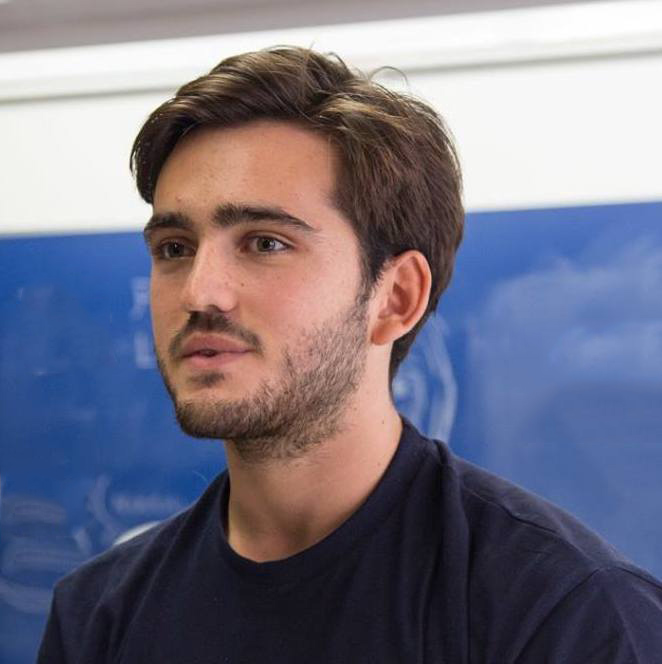
\includegraphics[width=3.5cm]{img/carlos_portrait.jpg}
\end{minipage} \hfill
\begin{minipage}{0.77\linewidth}
    \justifying{My name is \textbf{Carlos Segarra}. I am a 22 year old student from Barcelona. I am undergoing a double degree program at \textbf{CFIS} where I am studying \textbf{Mathematics} and \textbf{Telecommunications Engineering}. I am also a trainee at the Security Group at \textbf{Nokia Bell Labs} in Paris, France. In my spare time I train for amateur \textbf{triathlons}, I \textbf{read} and I love \textbf{learning new stuff}. \\[7pt]
\begin{tabular}{C{3cm}C{3cm}C{3cm}}
	\href{https://www.linkedin.com/in/carlossegarrag/}{\XeTeXLinkBox{
\includegraphics[width=1cm]{img/linkedin.jpg}}} & \vspace{-5pt} \href{https://github.com/csegarragonz}{\XeTeXLinkBox{
\includegraphics[width=1cm]{img/git.png}}} & \vspace{-8pt} \href{mailto:carlossegarragonzalez@gmail.com}{\XeTeXLinkBox{
\includegraphics[width=1cm]{img/mail.png}}}
\end{tabular}

\par}
\end{minipage}
\end{table}

\section{Education}

\begin{table}[h!]
\begin{tabular}{R{3cm}L{9.5cm}C{3cm}}	
\textsc{January} 2019 & B.Sc in \textsc{Mathematics} &  \multirow{2}{*}{\href{http://www.upc.edu/en}{\XeTeXLinkBox{
\includegraphics[width=1cm]{img/logoUPC.png}}}}\\[3pt] & \textbf{Technical University of Catalonia}, UPC & \\[7pt]

\textsc{January} 2019 &  B.Sc in \textsc{Telecommunications Science and Technology}&  \multirow{2}{*}{\href{http://www.upc.edu/en}{\XeTeXLinkBox{
\includegraphics[width=1cm]{img/logoUPC.png}}}} \\[3pt] & \textbf{Technical University of Catalonia}, UPC&  \\[7pt]

\textsc{January} 2019 &  Degree in \textsc{Multidisciplinar Engineering} &  \multirow{2}{*}{\href{http://www.cfis.upc.edu/en}{\XeTeXLinkBox{
\includegraphics[width=1cm]{img/cfis.png}}}} \\[3pt] & \textbf{CFIS}, Technical University of Catalonia\\[7pt]

\textsc{May} 2014 & Spanish Baccalaureate. Graduated with honors.  & \multirow{2}{*}{\href{http://www.betania-patmos.org/en/}{\XeTeXLinkBox{
\includegraphics[width=2cm]{img/bp.png}}}} \\[3pt] & \textbf{Betània-Patmos School}, Barcelona & \\[3pt]\end{tabular}
\end{table}


%----------------------------------------------------------------------------------------
%	WORK EXPERIENCE 
%----------------------------------------------------------------------------------------
\vspace{-5pt}


\section{Work Experience}
%
\begin{tabular}{R{3cm}|L{12.5cm}L{2cm}}
    \emph{Current} & Trainee at \textsc{CSEM} & \hspace{-102pt} \href{https://www.csem.ch/}{\XeTeXLinkBox{
\includegraphics[width=3cm]{img/csem}}} \\[3pt]
\textsc{October 2018} & \emph{Embedded Software Division} - Sup. Ricard Delgado Gonzalo, PhD & \\[3pt] 
& {\justifying\footnotesize{Dr Signorini and Pontecorvi work within the Cybersecurity department at Nokia Bell Labs in Paris-Saclay, France. Under their supervision, I worked in Bitcoin's Blockchain security. We defined, designed and implemented a modelling scheme for strange transaction chains. With this abstraction model we identified servicies within the Bitcoin ecosystem and we applied it to identity-oriented address clustering. }\par} &
\end{tabular}

\begin{tabular}{R{3cm}|L{12.5cm}L{2cm}}
    \emph{September 2018} & Trainee at \textsc{Nokia Bell Labs} & \hspace{-102pt} \href{https://www.bell-labs.com/}{\XeTeXLinkBox{
\includegraphics[width=3cm]{img/bell-labs}}} \\[3pt]
\textsc{June 2018} & \emph{Security Group} - Sup. Matteo Signorini, PhD and Matteo Pontecorvi, PhD & \\[3pt] 
& {\justifying\footnotesize{Dr Signorini and Pontecorvi work within the Cybersecurity department at Nokia Bell Labs in Paris-Saclay, France. Under their supervision, I worked in Bitcoin's Blockchain security. We defined, designed and implemented a modelling scheme for strange transaction chains. With this abstraction model we identified servicies within the Bitcoin ecosystem and we applied it to identity-oriented address clustering. }\par} &
\end{tabular}

\begin{tabular}{R{3cm}|L{12.5cm}L{2cm}}
\emph{June 2018} & Research Student at \textsc{Barcelona Supercomputing Center} & \hspace{-62pt} \href{https://www.bsc.es/}{\XeTeXLinkBox{
\includegraphics[width=1cm]{img/bsc}}} \\[3pt]
\textsc{April 2017} & \emph{Workflows and Distributed Computing Group} - Sup. Rosa M. Badia, PhD & \\[3pt] 
& {\justifying\footnotesize{The workflows and distributed computing group at BSC develops a programming framework, \href{https://www.bsc.es/research-and-development/software-and-apps/software-list/comp-superscalar/}{COMPSs}, which aims to ease the development of applications for distributed architectures. During my work there, I developed clustering algorithms in the Python binding of the software to test the scalability of the framework as well as new functionalities. All the executions were performed in the Mare Nostrum 4 supercomputer, enabling the use of bigger datasets and greater computational resources.}\par}
\end{tabular}
%------------------------------------------------

%----------------------------------------------------------------------------------------
%	EXTRACURRICULAR COURSEWORK
%----------------------------------------------------------------------------------------


\section{Extracurricular Coursework}
\begin{tabular}{R{3cm}L{9cm}C{3cm}}	
\textsc{September} 2017 &  Course in \small{\textsc{Bitcoin and Cryptocurrency Technologies}} & \hspace{15pt} \multirow{2}{*}{\href{https://www.coursera.org/learn/cryptocurrency}{\XeTeXLinkBox{
\includegraphics[width=2cm]{img/coursera.png}}}}\\[3pt]
 & University of \textbf{Princeton}, Coursera\\[7pt]
 
\textsc{March} 2017 &  Course in \textsc{Machine and Deep Learning} & \hspace{15pt} \multirow{2}{*}{\href{http://www.upc.edu/en}{\XeTeXLinkBox{
\includegraphics[width=1cm]{img/logoUPC.png}}}}\\[3pt] & \textbf{CFIS}, Technical University of Catalonia   \\[7pt]

\textsc{January} 2017 &  Course in \textsc{Machine Learning}  & \hspace{15pt} \multirow{2}{*}{\href{https://www.coursera.org/learn/machine-learning}{\XeTeXLinkBox{
\includegraphics[width=2cm]{img/coursera.png}}}}\\
& University of \textbf{Stanford}, Coursera \\[7pt]

\textsc{Summer} 2015 & Module in \textsc{Smartphone Applications} and & \hspace{15pt} \multirow{2}{*}{\href{http://robotics.leeds.ac.uk/}{\XeTeXLinkBox{
\includegraphics[width=2cm]{img/leeds.png}}}}\\
& \textsc{Introduction to Robotics} \\
 & Summer student at the \textbf{University of Leeds}, U.K\\[3pt]
\end{tabular}
%----------------------------------------------------------------------------------------
%	SCHOLARSHIPS AND ADDITIONAL INFO
%----------------------------------------------------------------------------------------
%\vspace{-5pt}
%
%\section{Scholarships and Certificates}
%
%\begin{tabular}{rl}
%\textsc{May} 2015 & Partial tuition fee for the Sudy Abroad \footnotesize (CFIS) \normalsize \\
%\textsc{January} 2015 & Economical reward for University Acces Exams \\
% &  (Fundació Catalunya Caixa - La Pedrera) \\
%\textsc{June} 2014 & BSc in Mathematics full tuition scolarship
%	\footnotesize (CFIS) \normalsize \\
%\textsc{May} 2014 & First University Year Scholarship \footnotesize(Generlitat de Catalunya)\normalsize\\
%\textsc{March} 2014 & Certificate in Advanced English \footnotesize (Grade A, 84/100) \normalsize \\
%\textsc{June} 2012 & Zertifikat A2 (German language) \footnotesize (Grade: 75/80) \normalsize \\
%\end{tabular}

%----------------------------------------------------------------------------------------
%	LANGUAGES
%----------------------------------------------------------------------------------------


\section{Languages}

\begin{tabular}{R{3cm}L{10cm}C{2cm}}
\textsc{English:} & \textbf{Certificate in Advanced English} & \multirow{2}{*}{
\includegraphics[width=1cm]{img/uk}} \\
 & Proficient level equivalent to a C2 due to a grade over 80. & \\
& & \\
\textsc{German:} & \textbf{Zertifikat A2} & \multirow{2}{*}{
\includegraphics[width=1cm]{img/german}} \\
 & Fluent. At level B1+ as of mid 2017. Capable of working in a German speaking environment. \\
 & & \\[-5pt]
\textsc{French:} & Basic Knowledge & 
\includegraphics[width=1cm]{img/french} \\
& & \\[-5pt]
\textsc{Spanish:} & \textbf{Native competence} & 
\includegraphics[width=1cm]{img/spain} \\
 & & \\[-7pt]
\textsc{Catalan:} & \textbf{Native competence} & 
\includegraphics[width=1cm]{img/catalan.png} \\
\end{tabular}

%----------------------------------------------------------------------------------------
%	COMPUTER SKILLS 
%----------------------------------------------------------------------------------------


\section{Technical Skills \& Research Interests}

\begin{tabular}{R{3cm}L{12cm}}
\textsc{ML \& DS}:  & 	\textbf{Machine Learning and Data Science} \\
& {\justifying Very good knowledge of Python applied to machine learning applications dealing with large amounts of data. \\
 Good knowledge of Matlab applied to both machine learning and signal processing.  \\
 Knowledge of R and AMPL for mathematical and statistical modelling. \par}  \\
 
\textsc{HPC}: & \textbf{High Performance Computing} \\
  & {\justifying Capable of working in high performance architectures such as clusters and grids. Know how to work with slurm and other queueing systems as well as with distributed file systems such as GPFS or HDFS. \par} \\
\textsc{Algorithmics}: &  Good knowledge of C++ and Java for multi-thread programming. \\
 & \\[-3pt]

 \textsc{R\&D Interests}: & Cybersecurity and Criptography. IoT, decentralised applications and \\ & Blockchain. Functional Programming. \\
 & \\[-3pt]
\end{tabular}

%\section{Skills and Relevant Coursework}
%\begin{tabular}{rl}
%\textsc{Mathematics:} & Discrete Mathematics, Probability, Algebra \\
%\textsc{Computer Science:} & Algorithmics, Object Oriented Programming,  Network Application And Services \\ &
% Introduction to Communications, Machine Learning \\
%\end{tabular}

%----------------------------------------------------------------------------------------
%	INTERESTS AND ACTIVITIES
%----------------------------------------------------------------------------------------
%Nomes per CV més informals
%\section{Interests and Activities}
%
%\begin{tabular}{rl}
%Sport: & really sportive person. Practice all kinds of sports almost on a daily basis. \\
%Literature: & interested in the theory of thought politics and philosophy in general. \\
%Teaching: & I consider teaching one of the best ways of learning and so I spend some of \\ & my free time helping younger students. \\
%Logical problems: & apart from my studies I also enjoy solving mathematical and logical puzzles \\ & aswell as programming in my spare time. \\
%
%	
%\end{tabular}

%----------------------------------------------------------------------------------------

\newpage

%----------------------------------------------------------------------------------------
%	GRADE TABLES
%----------------------------------------------------------------------------------------

%\par{\centering\Large \hypertarget{grds}{Master of Science in \textsc{Finance}}\par}\large{\centering Grades\par}\normalsize
%
%\begin{center}
%\begin{tabular}{lcc}
%\multicolumn{1}{c}{\textsc{Exam}} & \textsc{Grade}&\textsc{Credit Hrs}\\ \hline
%Corporate Finance (Valuation) & 25 & 6\\
%Financial Statement Analysis & 28 & 6\\
%Statistics & 27 & 6\\
%Theory of Finance & 26 & 6\\
%Quantitative Methods for Finance & 30 & 6\\
%Econometrics & 24 & 6\\
%Derivatives & 31 & 6\\
%Management of Financial and Insurance Companies & 30 & 6\\
%Business Law & 31 & 6\\
%Investment Banking	& 28 & 6\\ \\		
%Behavioral Models for Economics and Finance	 & 29 & 6\\
%Numerical Methods for Finance & 29 & 6\\
%Advanced Derivatives & 30 & 6\\
%Fixed Income (Advanced Methods) & 30 & 6\\ \\
%English Language & 30 &	4\\
%French Language & 31 &	4\\	
%Internship & & 8\\		
%Final Thesis & & 20\\	
%& Total & 120\\\cline{2-3}
%&\textsc{Gpa}&\textbf{8.0}
%\end{tabular}
%\end{center}
%\bigskip
%\hrule
%\bigskip
%
%%------------------------------------------------
%
%\bigskip
%
%\par{\centering\Large \hypertarget{grds_usc}{Exchange Program at \textsc{usc}, Los Angeles}\par}\large{\centering Grades\par}\normalsize
%
%\begin{center}
%\begin{tabular}{lcc}
%\multicolumn{1}{c}{\textsc{Exam}} & \textsc{Grade} & \textsc{Grade Points}\\ 
%\hline
%Corporate Financial Strategy & A & 4\\
%Derivatives & A & 4\\
%Money, Credit, and Banking & A & 4\\
%Business Strategy & A- & 3.5\\
%& &\\\cline{2-3}
%& \textsc{Gpa} & \textbf{3.875}
%\end{tabular}
%\end{center}

%----------------------------------------------------------------------------------------


\end{document}
